\documentclass[a4paper,12pt]{article}
\usepackage[pdfborder={0 0 0}]{hyperref}
%%\usepackage[defaultsans]{droidsans}
%%\renewcommand*\familydefault{\sfdefault} %% Only if the base font of the document is to be typewriter style
\usepackage[T1]{fontenc}
\usepackage[francais]{babel}
\usepackage[utf8]{inputenc}
\usepackage{color}
\usepackage{lmodern}
\usepackage{amsmath}
\usepackage{amssymb}
\usepackage{mathrsfs}
% \usepackage{pdfpages}
\usepackage{graphicx}
\usepackage[top=2.5cm, bottom=3cm, left=2cm, right=2cm]{geometry}
\usepackage{variations}
\usepackage{colortbl}
\usepackage{textcomp}
\usepackage{eurosym}
\usepackage{tabularx}
\usepackage{lastpage}
\usepackage{fancyhdr}

\pagestyle{fancy}

\fancyfoot[L]{\textit{IPIWolf}}
\fancyfoot[R]{\textit{Documentation technique}}
\fancyfoot[C]{\textit{Page \thepage/\pageref{LastPage}}}


\begin{document}
\title{Documentation utilisateur d'IPIWolf}
\author{Vincent Stébé - Nicolas Adam}
\date{Juin 2015}

\maketitle

\newpage 
\newgeometry{top=2cm, bottom=2cm}

\tableofcontents
\vspace{1cm}
\restoregeometry
\newpage

\section{Présentation}
\subsection{Le logiciel \emph{IPIWolf}}
Le logiciel \emph{IPIWolf} permet de traiter des fichiers issus d'accéléromètres.
Il prend en entrée des fichiers (appelés \emph{Raw File}) du format suivant :
\begin{verbatim}
$File has 224955801 lines.                                                                                                                            
Logger date      Logger time     N       N prime         X       Y       Z 
15/05/2014      08:00:01        28      1       -0.141  -1.609  1.531
                                -0.109  -0.078  1.016
                                -0.109  -0.078  1.016
                                -0.094  -0.078  1
                                -0.094  -0.078  1.016
                                -0.094  -0.078  1
                                -0.094  -0.078  1.031
                                -0.094  -0.062  1.016
(***)
\end{verbatim}
Le logiciel lit alors ce fichier et permet de sélectionner une partie du signal en spécifiant une date de début et une date de fin.
Il permet ensuite de rééchantillonner ce signal avec une fréquence de votre choix, et de procéder à un filtrage de fréquence.

\subsection{Configuration système}
Le logiciel a été conçu sous GNU/Linux (distributions Ubuntu et ArchLinux).
Il est nécessaire d'installer les dépendances suivantes :
\begin{itemize}
 \item Qt SDK 5.4
 \item FFTW 3
\end{itemize}
Ces librairies fonctionnent sur la plupart des systèmes.
Pour compiler, il suffit ensuite soit d'utiliser \emph{QtCreator} soit d'ouvrir un terminal et d'exécuter les commandes suivantes :
\begin{verbatim}
 qmake
 make
\end{verbatim}
L'exécutable \emph{ipiwolf} est alors généré et prêt à être utilisé.

\section{Utilisation}
\subsection{Ré-échantillonnage}
\subsubsection{Entrée des paramètres}
Appuyer sur le bouton \emph{Open Raw File} pour sélectionner un fichier à ré-échantillonner.
Choisir les différents paramètres de ré-échantionnage.
\begin{itemize}
 \item \textbf{Frequency} : Sélection de la fréquence de ré-échantionnage.
 \item \textbf{Start} : Sélection de la date à partir de laquelle commencera le ré-échantionnage.
 \item \textbf{End} : Sélection de la date à partir de laquelle finira le ré-échantionnage.
\end{itemize}
\begin{center}
 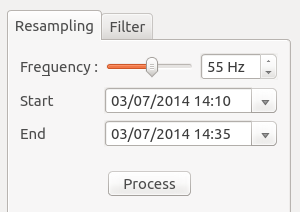
\includegraphics[width=6cm]{img/param_resampling.png}
\end{center}
Il suffit enfin d'appuyer sur bouton \emph{process} pour lancer le calcul du ré-échantillonnage. Une fenêtre de chargement s'affichera 
pour permettre de suivre la progression du calcul.


\subsubsection{Visualisation des données}
L'onglet \emph{Signal} permet de visualiser la courbe des données ré-échantionnées.
Plusieurs boutons permetent de sélectionner les informations à afficher.
\begin{itemize}
  \item \textbf{X} : Affiche la courbe des déplacements sur l'axe X.
  \item \textbf{Y} : Affiche la courbe des déplacements sur l'axe Y.
  \item \textbf{Z} : Affiche la courbe des déplacements sur l'axe Z.
  \item \textbf{XYZ} : Affiche la courbe de la norme de chaques points. Calcul : $\sqrt{x^2 + y^2 + z^2}$
\end{itemize}

\begin{center}
 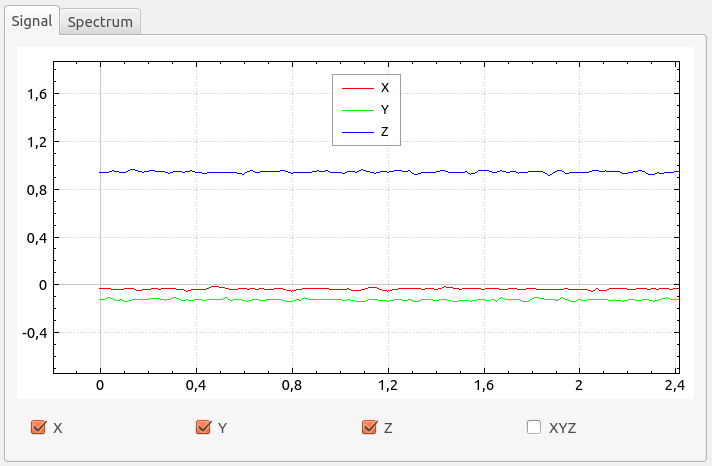
\includegraphics[width=17cm]{img/signal_graph.png}
\end{center}


\subsection{Filtrage de fréquence}
Pour filtrer une signal, il faut utiliser un signal bien échantillonné.
Vous devez donc :
\begin{itemize}
 \item soit ouvrir un fichier issu du capteur (\emph{Open Raw File}) et le rééchantillonner (voir la partie précédente)
 \item soit ouvrir un fichier déjà rééchantilloné (\emph{Open Resampled File})
\end{itemize}
\subsubsection{Visualisation du spectre}
Il est possible de visualiser le spectre avant de procéder au filtrage. 
Ouvrir l'onglet \emph{Spectrum} et choisissez les axes à traiter en bas de la fenêtre
Vous obtenez alors un graphe comme celui-ci (un seul axe traité) :


\subsubsection{Filtrage du signal}
Le filtrage se fait sur trois paramètres :
\begin{itemize}
 \item \emph{Threshold} : correspond à la fréquence de coupure
 \item \emph{Direction} : définit si le filtre est un passe-bas \emph{(LOW)} ou passe-haut \emph{(HIGH)}
 \item \emph{Axes} : définit l'axe à filtrer
\end{itemize}
Par exemple, un filtrage avec les paramètres suivants :
\begin{center}
 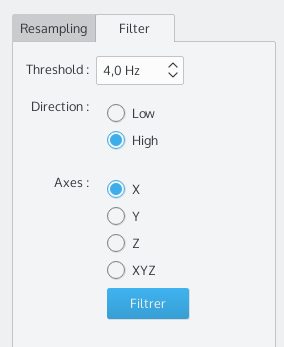
\includegraphics[width=5cm]{img/filterParams.png}
\end{center}
On a un filtre passe-haut sur l'axe X avec une fréquence de coupure de 4Hz. On obtient, après avoir à nouveau généré le spectre :
\begin{center}
 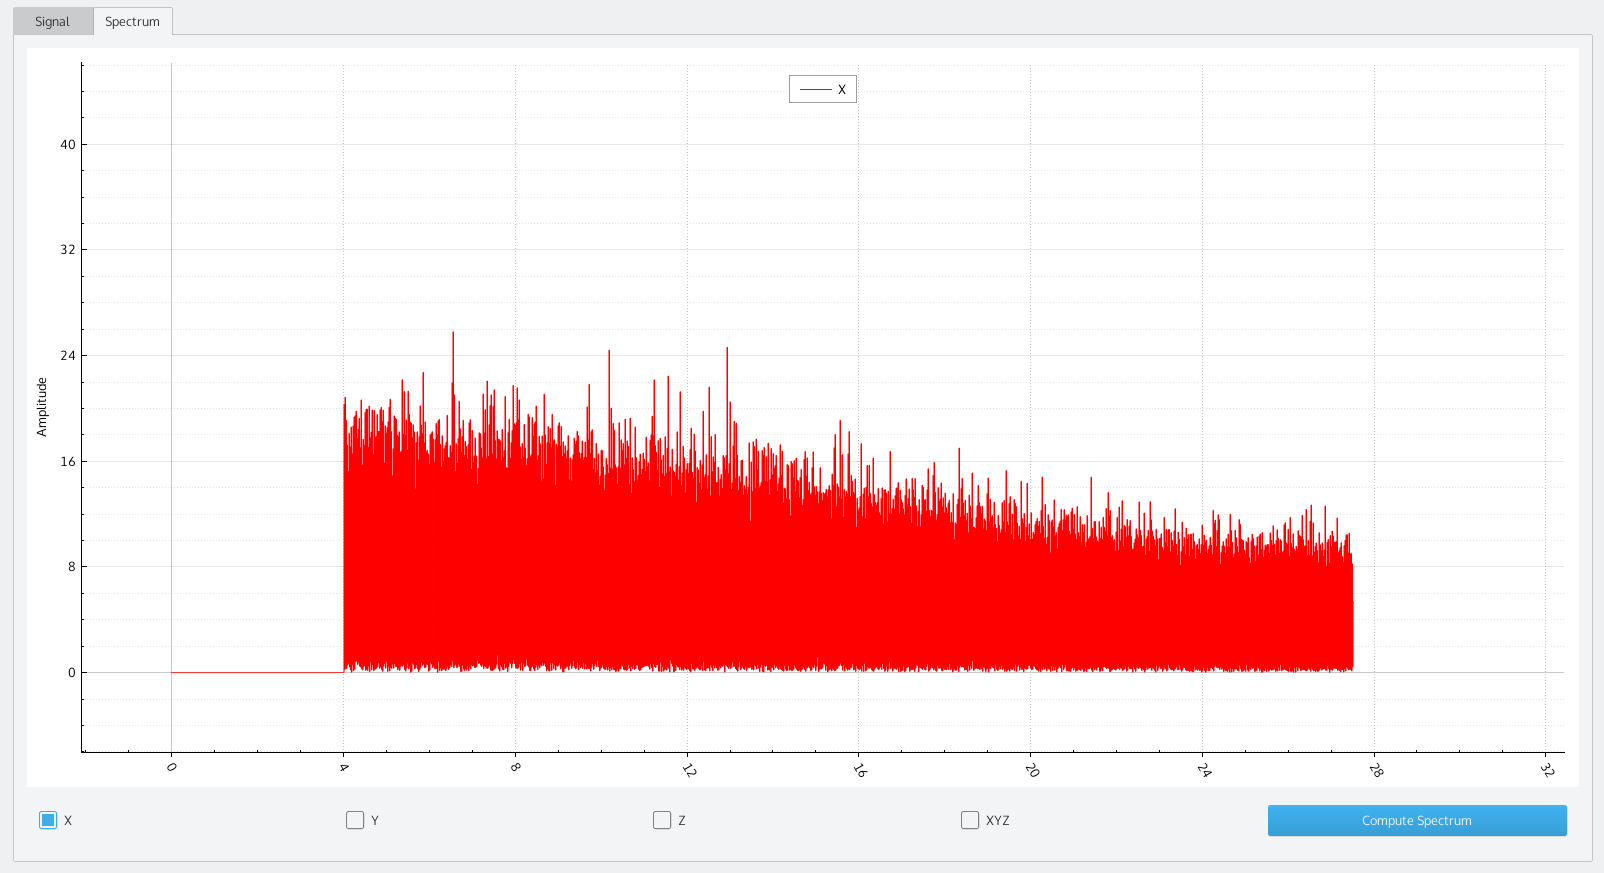
\includegraphics[width=17cm]{img/filteredSpectrum.png}
\end{center}
Vous pouvez désormais retourner sur l'onglet \emph{signal} et visualiser le nouveau signal. Vous pouvez sauvegarder celui-ci avec le bouton \emph{Save file}.

\end{document}

